\section{Conception}
    \subsection{Opérations importantes}
    \begin{itemize}
        \item a) Commandes/Ventes de plateau
        \item c) Approvisionnement et stockage
    \end{itemize}


\paragraph{Datamarts} 
    \begin{figure}[h]
        \centerline{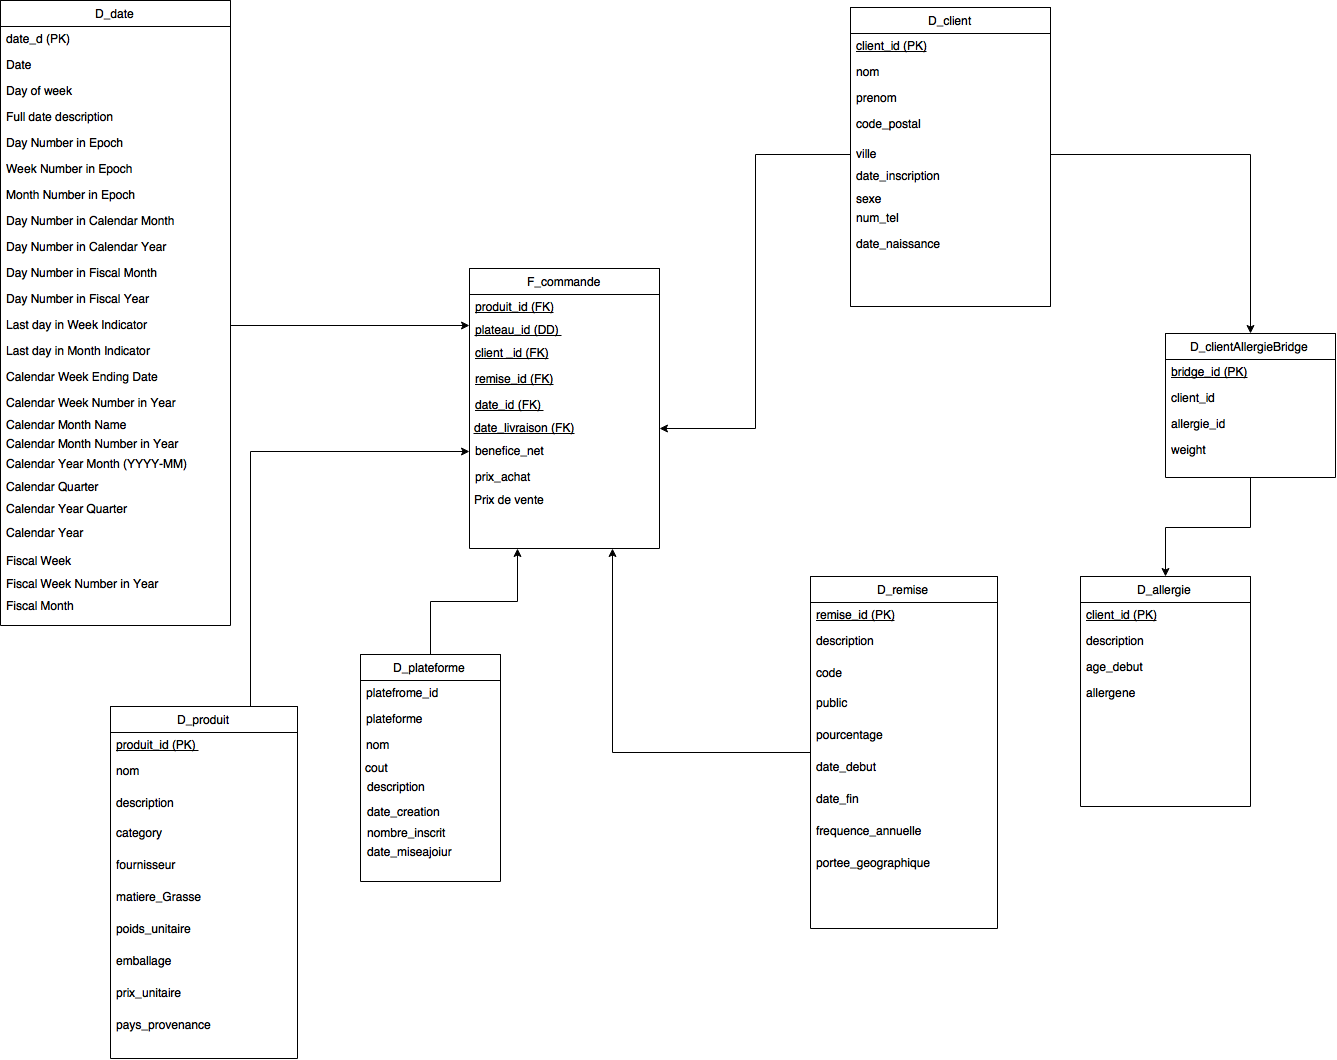
\includegraphics[scale=0.4]{EtoileDM1.png}}
        \caption{Premier Datamart}
        \label{fig:UML}
    \end{figure}
    
    \begin{figure}[h]
        \centerline{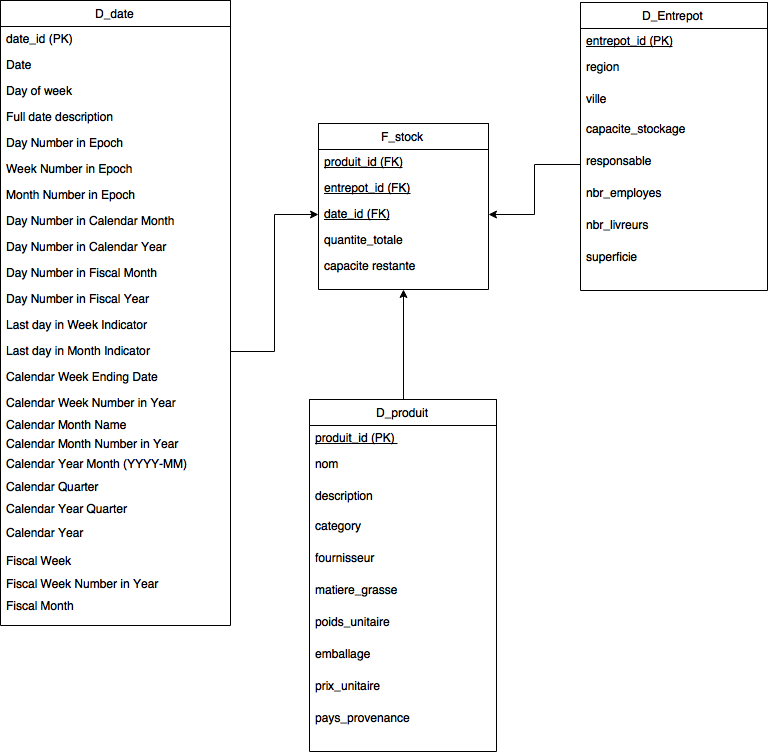
\includegraphics[scale=0.6]{EtoileDM2.png}}
        \caption{Deuxième Datamart}
        \label{fig:UML}
    \end{figure}

\paragraph{} Les mesures : Prix\_Achat et Prix\_Vente et Benefice\_Net sont toutes trois additives.

\paragraph{} 
\paragraph{} Datamart opération c :
Il s’agit d’un snapshot périodique.
La mesure de capacité restante est semi-additive.

\subsection{Réponse aux requêtes} 
\paragraph{} Le datamart ayant changé, on ne peut pas interroger la DW avec les traitements prévus précédemment, voir nouveaux traitement dans la partie réalisation

\subsection{Détails}

\paragraph{} La notion de plateau était celle présente dans notre modèle objet-relationnel, et qui consiste en un regroupement de produits constituant un repas commandé.
\paragraph{} En raison de la granularité différente de notre entrepôt (plus détaillée/Transaction concernant un seul produit et non un plateau), la majorité des attributs de la table plateau ont migré vers la notion atomique de produit. La dimension associée est ainsi devenue superflue.
\paragraph{} Il reste néanmoins utile d’identifier les produits achetés au sein d’une même commande. 
\paragraph{} Afin de permettre cela, nous décidons de mettre l’attribut  "plateau\_id" dans la table de fait "F\_commande". Il devient donc possible de retrouver les associations de produits (produits commandés ensemble), en regroupant les commandes ayant la même valeur de "plateau\_id".

    \begin{figure}[h]
        \centerline{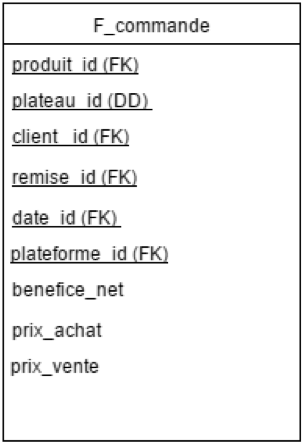
\includegraphics[scale=0.6]{TableFCom}}
        \caption{Table de fait F\_Commande}
        \label{fig:UML}
    \end{figure}
